In this section, a description of the system-to-be is provided following the World and Machine model introduced by Jackson and Zave~\cite{w&m}.

In their model, they indicate as the \textit{Machine} the product-to-be. The \textit{Machine} domain is the set of phenomena that the machine can control: data structures it can manipulate, algorithms it can run, devices it can
control, inputs it can get from the world, and so on.

In contrast, the \textit{World} domain is the real-life context into which the \textit{Machine} will be introduced, and in particular, is that part of the world in which the \textit{Machine}’s actions will be observed and evaluated.

The \textit{World} and the \textit{Machine} are connected, because the second must interact with the first in order to be useful. The connection is via \textit{Shared Phenomena} – things that are observable both by the \textit{Machine} and by the \textit{World}. \textit{Shared Phenomena} include events in the real world that the \textit{Machine} can directly sense and actions in the real world that the \textit{Machine} can directly cause.

\begin{figure}[H]
\begin{center}
		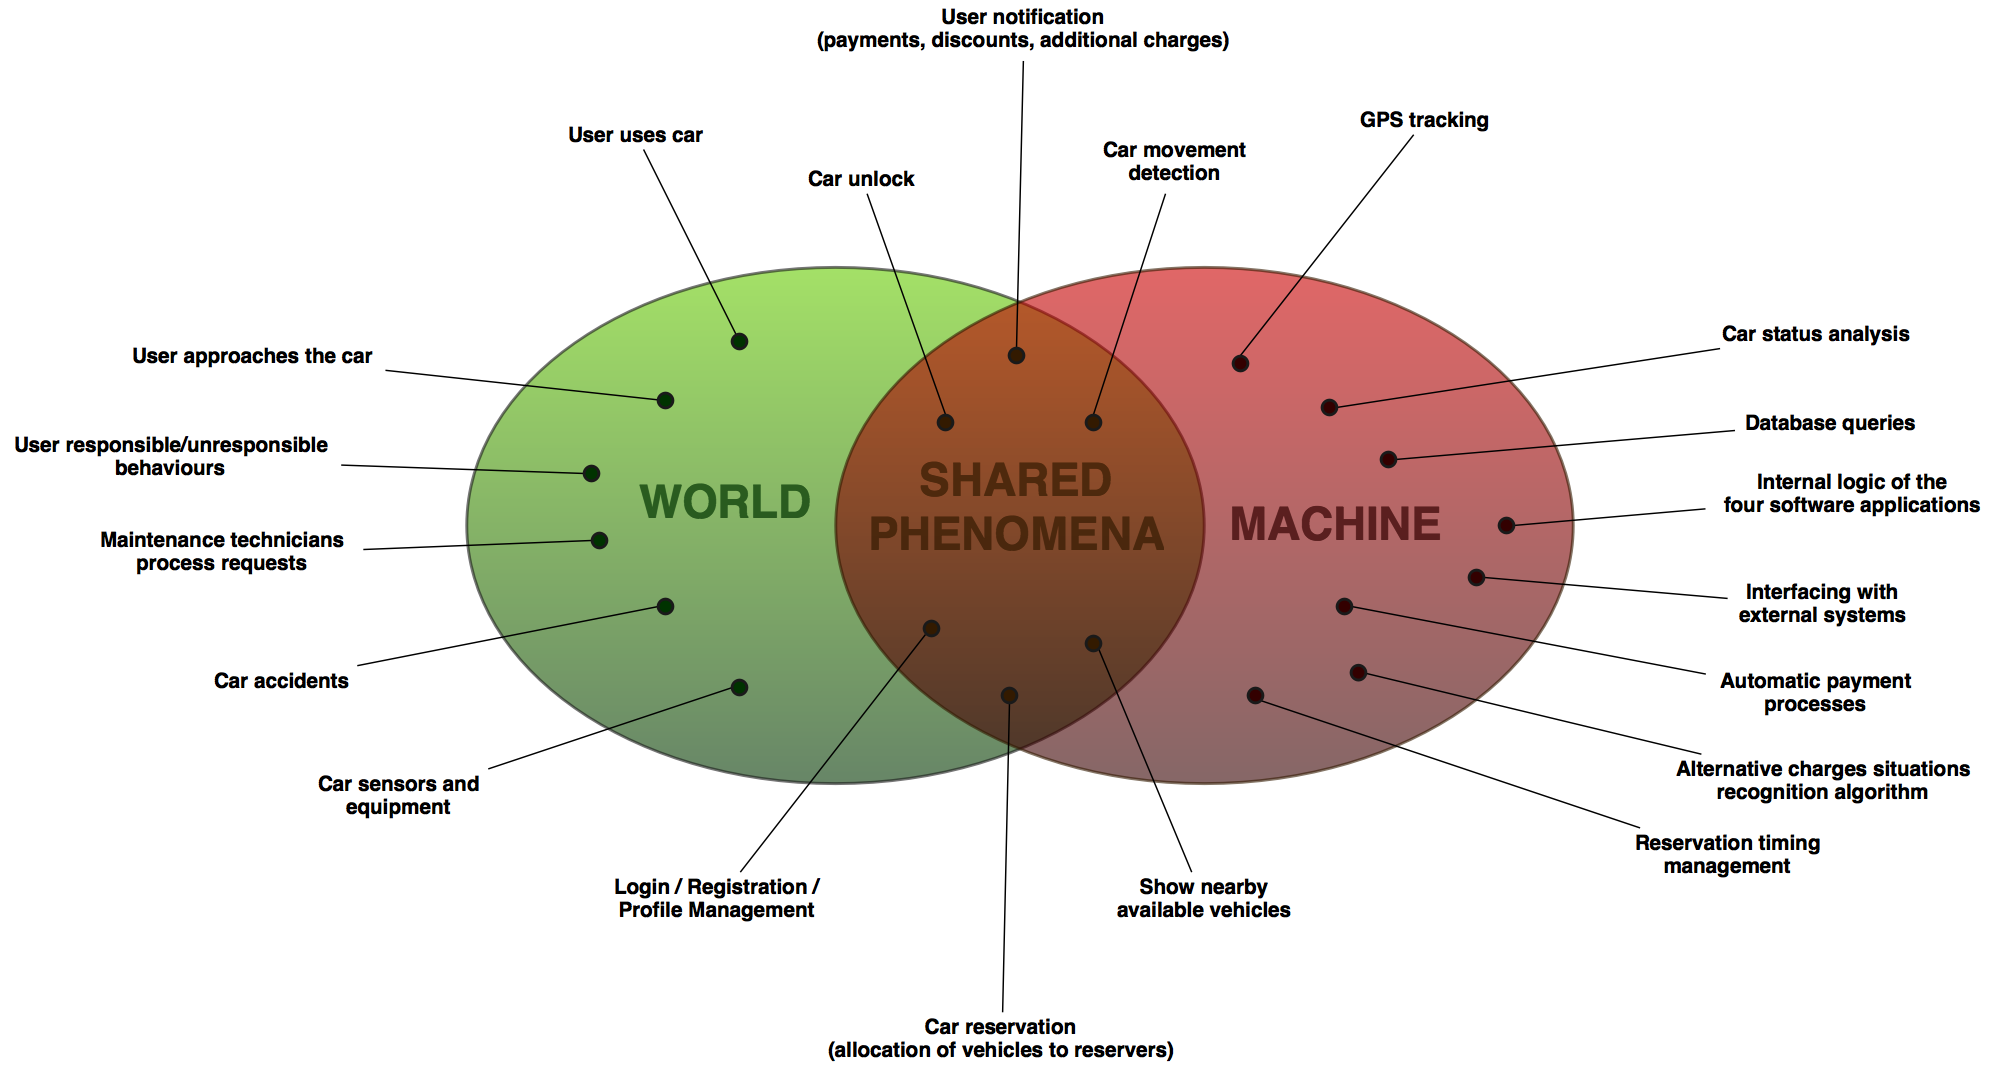
\includegraphics[width=\textwidth]{./pictures/World_and_Machine.png}
		\caption{World and Machine model for the main functionalities to be provided by the system.}
		\label{class_diagram}
\end{center}
\end{figure}